\documentclass{article}
\usepackage{graphicx}
\usepackage{verbatim}
\usepackage{dcolumn}
\usepackage{array}
\usepackage{mathtools}
\usepackage{float}
\usepackage{booktabs}
\usepackage{cleveref}
\usepackage{siunitx}
\usepackage{enumitem}
\usepackage{bbm}
\usepackage{xcolor}
\usepackage{amsmath}
\usepackage{amsfonts}
\usepackage{amsthm}
\usepackage{amssymb}
\usepackage{booktabs}
\usepackage{caption}
\usepackage{float}
\usepackage{natbib}
\newtheorem{assump}{Assumption}[section]
\newtheorem{lemma}{Lemma}[section]
\newtheorem{corollary}{Corollary}[section]
\newtheorem{theorem}{Theorem}[section]
\usepackage[toc,page]{appendix}
\pagestyle{plain}
\topmargin 0.0cm
\oddsidemargin 0.2cm
\textwidth 16cm
\textheight 21cm
\footskip 1.0cm
\title{A Dynamic Panel Data Framework for Identification and Estimation of Nonlinear Production Functions}
\author{Justin Doty\thanks{Department of Economics, University of Iowa, S321 Pappajohn Business Building, 21 E Market St, Iowa City, IA 52242. Email: \texttt{justin-doty@uiowa.edu}}
}
\date{\vspace{-5ex}}
\begin{document}
\maketitle{}

\begin{abstract}
This paper studies identification and estimation of a non-linear model for production functions with unobserved heterogeneity. Non-parametric identification results are established for the production function under stationarity assumptions. This paper then estimates the conditional quantiles of firm production using non-linear quantile regression. This paper finds that objects of interest, such as output elasticities with respect to inputs vary considerably with respect to the rank of unobserved technology shocks. In the application to US firm-level manufacturing data, this paper considers a Translog production function with non-Hicksian neutral productivity shocks and a productivity process that features non-linear persistence.
\end{abstract}

\section{Introduction}

\section{Literature Review}

\section{The Model of Firm Production} \label{model}

\subsection*{Output}
Consider a nonlinear model for a firm's gross-output production function (in logs)
\begin{equation}\label{modelY}
y_{it}=f_{t}(k_{it}, l_{it}, m_{it}, \omega_{it}; \beta(\eta_{t}))
\end{equation}
where $y_{it}$ is firm $i$'s output at time $t$ and $l_{it}, m_{it}, k_{it}$ denotes optimal input choices for labor, materials, and capital respectively. The unobserved productivity is denoted by $\omega_{it}$ which is correlated to input choices of the firm at time $t$. I let the output elasticities $\beta$ be functionally dependent on unobserved production shocks $\eta_{i1},\dots, \eta_{iT}$ which are independent of input choices and productivity at time $t$.\\

Without loss of generality I normalize $\eta_{it}\sim U[0,1]$. This model corresponds to a nonlinear random coefficient model where the outcome $y_{it}$ is assumed to be strictly monotonic in $\eta_{it}$. In practice I can allow for nonlinear interactions between inputs and unobserved productivity at different quantiles so that marginal effects can be modeled as non-Hick's neutral. For empirical simplicity I can model separability in the unobserved productivity to calculate total factor productivity (TFP). The function $f_{t}$ is an unknown nonlinear function.

In this model, heterogeneity in production technology across firms is driven by the rank of the unobserved production shocks $\eta_{it}$. I specify the following functional forms for the input demand functions.

\subsection*{Labor} 
Labor inputs are chosen to maximize current period profits and therefore are a function of current period state variables
\begin{equation} \label{modelL}
l_{it}=\ell_{t}(k_{it}, \omega_{it}; \alpha_{l}(\epsilon_{it}))
\end{equation}
where $\epsilon_{it}$ is iid and independent of current period state variables. I assume the labor demand function $\ell$ is strictly increasing in $\epsilon_{it}$ which is normalized to be uniformly distributed on the interval $[0,1]$

\subsection*{Materials} 
Material inputs are chosen to maximize current period profits and therefore are a function of current period state variables
\begin{equation} \label{modelM}
m_{it}=\mu_{t}(k_{it}, \omega_{it}, \alpha_{m}(\varepsilon_{it}))
\end{equation}
where $\varepsilon_{it}$ is iid and independent of current period state variables. I assume the materials demand function $\mu$ is strictly increasing in $\varepsilon_{it}$ which is normalized to be uniformly distributed on the interval $[0,1]$. I can extend this to the case where labor is chosen prior to choosing material inputs in which case I would include $l_{it}$ as a state variable in equation \eqref{modelM}.

\subsection*{Capital Accumulation}
Capital accumulates to the following generalized law of motion
\begin{equation} \label{modelK}
K_{it}=\kappa_{t}(K_{it-1}, I_{it-1}, \upsilon_{it-1})
\end{equation}
where $I_{it-1}$ denotes firm investment in the prior period. Under this specification, capital is determined in period $t-1$. I introduce a random error term $\upsilon_{it-1}$ which eliminates the deterministic relationship of capital with respect to previous period state and decision variables. I will show later that this step is crucial for my nonparametric identification result which is used by \cite{Hu2019}. I assume $\upsilon_{it}$ is independent of $\eta_{it}$ conditional on $(\omega_{it}, k_{it}, l_{it}, m_{it})$

\subsection*{Productivity}
Productivity evolves according to the exogenous first order Markov process:
\begin{equation}\label{modelw}
\omega_{it}=g_{t}(\omega_{it-1}; \rho(\xi_{it}))
\end{equation}

where $\xi_{i1},\dots, \xi_{iT}$ are independent uniform random variables which represent innovation shocks to productivity. I assume $\omega_{it}$ is monotonic in $\xi_{it}$ I let $g$ be another unknown nonlinear function that allows the persistence in productivity in firms to be nonlinear across different quantiles. The exogeneity of the productivity process can be relaxed when I consider productivity enhancing activities such as R\&D similar to \cite{Doraszelski2013}.

\subsection*{Investment} \label{investment}
I introduce a dynamic model of firm investment that is a slight modification of \cite{Ericson1995} which can also be found in \cite{Hu2013} and \cite{Ackerberg2007}. In each period, a firm chooses investment to maximize its discounted future profits:
\begin{equation} \label{valuefn}
I_{it}=I^{*}(K_{it}, \omega_{it}; \delta(\zeta_{it}))=\underset{I_{t}\geq 0}{\operatorname{argmax}}\Bigg[\Pi_{t}(K_{it}, \omega_{it}, \zeta_{it})-c(I_{it})+\beta\mathbbm{E}\big[V_{t+1}(K_{it+1}, \omega_{it+1}, \zeta_{it+1})|\mathcal{I}_{t}\big]\Bigg],
\end{equation}
Here, $\pi_{t}(\cdot)$ is current period profits as a function of the state variables and an unobservable demand shock $\zeta_{it}$. These are shocks to a firm's product demand which are privately observed by each firm and i.i.d across $i$ and $t$. I assume these shocks are independent from the firm's state variables. Current costs to investment are given by $c(I_{t})$ and $\beta$ is the firm's discount factor. \cite{Pakesa} provides specific conditions for which the investment policy function is strictly increasing in its unobservable components. Without loss of generality, I normalize $\zeta_{it}\sim U[0,1]$


%-----------------------------------------------------------------------------------------------------
\section{Identification}

I begin by listing preliminary assumptions regarding the main econometric restrictions of the model, some of which were informally stated in the previous section. Here, I focus on the restrictions on the production function.

\begin{assump} \label{pfmomentassume}
~
\begin{enumerate}[label=(\roman*)]
    \item $\eta_{it}$ follows a standard uniform distribution independent $\mathcal{I}_{it}$, where $\mathcal{I}_{it}$ denotes the firm $i's$ information set at time $t$
    \item The production function $y_{it}=f_{t}(k_{it}, l_{it}, m_{it}, \omega_{it}, \beta(\eta_{t}))$ is strictly increasing in $\eta_{it}$
    \item $\eta_{it}$ is independent and identically distributed across firms and time
    \end{enumerate}
\end{assump}

Then, according to Assumption \ref{pfmomentassume} the following moment restriction holds:
\begin{equation}
\mathbbm{E}_{nT}[\Psi_{\tau}(y_{it}-f_{t}(k_{it}, l_{it}, m_{it}, \omega_{it}; \beta(\tau)))|\mathcal{I}_{it}]=0,
\end{equation}
where $\Psi_{\tau}(u)=\mathbbm{1}\{u\leq0\}-\tau$. Using the law of iterated expectations, the following unconditional integrated moment restriction can be written as
\begin{equation} \label{unconditional}
\mathbbm{E}_{nT}\bigg[\int[k_{it}, l_{it}, m_{it}, \omega_{it}]\Psi_{\tau}(y_{it}-f_{t}(k_{it}, l_{it}, m_{it}, \omega_{it}; \beta(\tau)))g_{i}(\omega^{T}_{i};\theta(\cdot))d\omega^{T}_{i}\bigg]=0,
\end{equation}
where $g_{i}(\omega^{T}_{i};\theta(\cdot))=f(\omega^{T}_{i}|y^{T}_{i}, k^{T}_{i}, l^{T}_{i}, m^{T}_{i}, I^{T}_{i};\theta(\cdot))$ denotes the posterior density of $\omega^{T}_{i}=(\omega_{it},\dots,\omega_{iT})$ which depends on the continuum of parameters $\theta(\cdot)=(\beta(\cdot), \alpha_{l}(\cdot), \alpha_{m}(\cdot), \rho(\cdot), \delta(\cdot))$. I only consider exact identification for the above moment restriction, but I include investment in the conditioning set of the posterior density to capture the capital accumulation process which depends on last periods investment decisions, here $I_{it}\in\mathcal{I}_{it}$. In my model the posterior density is:

\begin{equation}\label{posterior}
\begin{split}
g_{i}(\omega^{T}_{i};\theta(\cdot))& \propto\prod_{t=1}^{T}f(y_{it}|k_{it}, l_{it}, m_{it}, \omega_{it};\beta(\cdot))f(l_{it}|k_{it}, \omega_{it};\alpha_{l}(\cdot))f(m_{it}|k_{it}, \omega_{it};\alpha_{m}(\cdot)) \\
&\times f(i_{it}|k_{it}, \omega_{it};\delta(\cdot))\prod_{t=2}^{T}f(\omega_{it}|\omega_{it-1};\rho(\cdot))f(\omega_{i1};\rho_{1}(\cdot)),
\end{split}
\end{equation}
Therefore, the identification of the production function in \eqref{unconditional} relies on identification of the conditional densities of production, labor, materials, investment, and the productivity process\footnote{Note that since the capital accumulation process does not directly depend on productivity, it drops out of the conditioning density. Identifying the investment rule should be sufficient for identifying capital dependence on last period's productivity}. I show that these densities are nonparametrically identified using \cite{Hu2008}. To show this, I introduce some new notation. Let $Z_{t}=(l_{t}, k_{t}, m_{t}, k_{t+1})$ denote conditioning variables where I have dropped the $i$ subscript for convenience. Assume the following: 

\begin{assump} (Conditional Independence):\\ \label{conditionalindependence}
~
$f(y_{t}|y_{t+1}, I_{t}, \omega_{t}, Z_{t})=f(y_{t}|\omega_{t}, Z_{t})$ and
$f(I_{t}|y_{t+1}, \omega_{t}, Z_{t})=f(I_{t}|\omega_{t}, Z_{t})$
\end{assump}
The first equality of Assumption \ref{conditionalindependence} states that conditional on $\omega_{t}$ and $Z_{t}$, $y_{t+1}$ and $I_{t}$ do not provide any additional information about $y_{t}$. The second equality states that conditional on $\omega_{t}$ and $Z_{t}$, $y_{t+1}$ does not provide any additional information about $I_{t}$. These are satisfied by mutual independence assumptions on $\eta_{t}$ and $\zeta_{t}$ conditional on $(\omega_{t}, k_{t}, l_{t}, m_{t})$ and the fact that $\eta_{it}$ is assumed to be conditionally independent over time. The next assumption is more technical.

\begin{assump} \label{injectivity} (Injectivity): The operators $L_{y_{t}|Z_{t}, \omega_{t}}$ and $L_{y_{t+1}|Z_{t}, \omega_{t}}$ are injective
\end{assump}

The above assumption allows us to take inverses of the operators. Consider the operator $L_{y_{t}|Z_{t}, \omega_{t}}$, following \cite{Hu2008}, injectivity of this operator can be interpreted as its corresponding density $f_{y_{t}|Z_{t}, \omega_{t}}(y_{t}|Z_{t}, \omega_{t})$ having sufficient variation in $\omega_{t}$ given $Z_{t}$. This assumption is often phrased as completeness condition in the nonparametric IV literature on the density $f_{y_{t}|k_{t}, \omega_{t}}(y_{t}|Z_{t}, \omega_{t})$. More formally, for a given $Z_{t}\in Supp(Z_{t})$
\begin{equation}
\int f_{y_{t}|Z_{t}, \omega_{t}}(y_{t}|Z_{t}, \omega_{t})g(\omega_{t})d\omega_{t}=0
\end{equation}
for all $y_{t}$ implies $g(\omega_{t})=0$ for all $\omega_{t}$\\

For injectivity of the second operator $L_{y_{t+1}|Z_{t}, \omega_{t}}$ it is intuitive to consider $y_{t+1}$ having sufficient variation for different values of $\omega_{t}$ given $Z_{t}$. Since productivity is specified as an AR(1) process and is highly persistent over time, this assumption is intuitive. 

This assumption is more restrictive than that of \cite{Hu2019}. Since their model is separable in $\omega_{t}$ they are able utilize convolution type arguments which require mild conditional independence assumptions as well as assumptions regarding characteristic functions. Injectivity is the price we pay for assuming a more general production function specification. I also require two additional assumptions for uniqueness of the identification strategy.

\begin{assump} \label{uniqueness} (Uniqueness): For any $\bar{\omega}_{t}, \tilde{\omega}_{t}\in \Omega$, the set $\{f_{I|\omega, Z}(I_{t}|\bar{\omega}_{t}, Z_{t})\neq f_{I|\omega, Z}(I_{t}|\tilde{\omega}_{t}, Z_{t})\}$ has positive probability whenever $\bar{\omega}_{t}\neq\tilde{\omega}_{t}$
\end{assump}
This assumption is relatively weak and is satisfied if there is conditional heteroskedasticity in $f_{I|\omega, Z}$ or if any functional of its distribution is strictly increasing in $\omega_{t}$. For example, this assumption is satisfied if $E[I_{t}|\omega_{t},Z_{t}]$ is strictly increasing in $\omega_{t}$ which is similar to the invertibility conditions required in \cite{Olley1996}. This assumption is problematic if investment is censored, in which case $E[I_{t}|\omega_{t},Z_{t}]$ can only be inverted for positive values of investment. In this case we can consider for some. Therefore, I can assume $E[\mathbbm{1}\{I_{it}>0\}|\omega_{t},Z_{t}]$ as the functional that satisfies the monotonicity assumption.  Since I will estimate input decision rules in my model using quantile regression, correcting for censoring is straightforward as I will show later. However, in my application censoring is not an issue since I use publicly listed firms, most of which who report positive capital expenditure in their income statements.

\begin{assump} \label{normalization} (Normalization): There exists a functional $\Gamma$ such that $\Gamma[f_{y|\omega,Z}(y_{t}|\omega_{t}, Z_{t})]=\omega_{t}$
\end{assump}
This functional does not need to be known, it is sufficient to consider a known function of the data distribution as shown by \cite{Arellano2016}. For a general nonseparable panel model this assumption is satisfied if $E[y_{t}|\omega_{t}, Z_{t}]$ is strictly increasing in $\omega_{it}$, then one could normalize $\omega_{t}=E[y_{t}|\omega_{t}, Z_{t}]$. In my empirical application, we use a non-separable translog production function. In this case our normalization can be achieved by $E[y_{t}|\omega_{t}, 0]=\omega_{t}$. With these assumptions I can now state the first part of our identification results.

\begin{theorem} \label{idpart1} Under Assumptions \ref{conditionalindependence}, \ref{injectivity}, \ref{uniqueness}, and \ref{normalization}, given the observed density $f_{y_{t}, I_{t}|y_{t+1}, Z_{t}}$, the equation
\begin{equation}
f_{y_{t}, I_{t}|y_{t+1}, Z_{t}}(y_{t}, I_{t}|y_{t+1}, Z_{t})=\int f_{y_{t}|\omega_{t}, Z_{t}}(y_{t}|\omega_{t}, Z_{t})f_{I_{t}|\omega_{t}, Z_{t}}(I_{t}|\omega_{t}, Z_{t})f_{\omega_{t}|y_{t+1}, Z_{t}}(\omega_{t}|y_{t+1}, Z_{t})d\omega_{t}
\end{equation}
admits a unique solution for $f_{y_{t}|\omega_{t}, Z_{t}}, f_{I_{t}|\omega_{t}, Z_{t}}$ and $f_{\omega_{t}|y_{t+1}, Z_{t}}$
\end{theorem}
\textit{Proof:} See Appendix.\\

This result identifies the conditional density of output and investment. It also identifies the marginal distribution for productivity since $f_{\omega_{t}}=\int f_{\omega_{t}|y_{t+1}, Z_{t}}f_{y_{t+1},Z_{t}}d(y_{t+1},Z_{t})$ where $f_{y_{t+1},Z_{t}}$ is known from the observed data. It also identifies the input decision rules for the labor and material inputs. We need additional results to identify the productivity process $f_{\omega_{t}|\omega_{t-1}}(\omega_{t}|\omega_{t-1})$ and the initial condition $f_{\omega_{t-1}}(\omega_{t-1})$. The requirements for identifying these distributions are different if the production function is stationary or non-stationary. Therefore I claim two separate results.

\begin{corollary} \label{stationary} (Stationarity): Suppose that the production function is stationary i.e. $f_{y_{t}|\omega_{t}, Z_{t}}=f_{y_{1}|\omega_{1}, Z_{1}} \forall t\in\{1,\cdots,T\}$. Then, under Assumptions \ref{conditionalindependence}, \ref{injectivity}, \ref{uniqueness}, and \ref{normalization}, the observed density $f_{y_{t}, I_{t}|y_{t+1}, Z_{t}}$ uniquely determines the density $f_{\omega_{t+1}|\omega_{t}}$ and the initial condition $f_{\omega_{t}}$ for any $t\in\{1,\dots,T-1\}$
\end{corollary}
\textit{Proof:} See Appendix.\\
\begin{corollary} \label{stationary} (Non-Stationary): Under Assumptions \ref{conditionalindependence}, \ref{injectivity}, \ref{uniqueness}, and \ref{normalization}, the observed density $f_{y_{t+1}, I_{t+1}|y_{t+2}, y_{t} Z_{t+1}}$ uniquely determines the density $f_{\omega_{t+1}|\omega_{t}}$ and the initial condition $f_{\omega_{t}}$ for any $t\in\{1,\dots,T-2\}$
\end{corollary}
\textit{Proof:} See Appendix.\\

The main conclusion of these two corollaries state that under the condition of stationarity, the productivity process can be identified with $T=2$ observations per firms whereas under non-stationarity, the productivity process is identified with $T=3$ observations per firm. The number of time periods required for identification increases with the length of the auto-regressive process. It is standard to estimate an AR(1) process for productivity. The data requirements are similar to the control function approach where the instrument set often includes secondary lags of inputs. The main identification assumptions are stronger than those in \cite{Hu2019}, but necessary for the generality of the model I present in this paper.

%----------------------------------------------------------------------------------------------------------

\section{Estimation Strategy}

I specify the following functional forms for estimation of the model in Section \ref{model}.

\subsection*{Output:}
\begin{equation}\label{ymodel}
\begin{split}
Q_{t}(y_{it}|k_{it}, l_{it}, m_{it}, \omega_{it}, \tau)&=Q(y_{it}|k_{it}, l_{it}, m_{it}, \omega_{it}, t, \tau)\\
&=\beta_{0}(\tau)+\beta_{t}(\tau)t+\sum_{0<n_{x}\leq n}\beta_{n_{k}, n_{l}, n_{m}}(\tau)k_{it}^{n_{k}}l^{n_{l}}_{it}m^{n_{m}}_{it}\omega_{it}
\end{split}
\end{equation}
where $t$ denotes the age of firm $i$ at time $t$, $n_{x}=n_{k}+n_{l}+n_{m}$. In my application I take $n_{k}=n_{l}=n_{m}=2$. In this case the production function is specified as Translog with first-order interactions of productivity, in a sense, allowing for productivity to affect input usage beyond a Hicks-neutral effect. Therefore, I have a total of 21 parameters to estimate.

\subsection*{Labor Input:}
I specify the labor input demand equation as follows:
\begin{equation} \label{lmodel}
\begin{split}
Q_{t}(l_{it}|k_{it}, \omega_{it}, \tau)&=Q(l_{it}|k_{it}, \omega_{it}, t, \tau)\\
&=\sum_{j=1}^{J}\alpha_{l,j}(\tau)\psi_{l,j}(k_{it}, \omega_{it}, t)
\end{split}
\end{equation}
where $\psi_{l,j}$ is a tensor product linear sieve. One could use basis functions as Fourier, B-splines, or Hermite polynomials. In practice I approximate this function by a third-order polynomial with interactions in $\omega_{it}$ and $k_{it}$ and additive in firm age.

\subsection*{Materials Input:}
I specify the material input demand equation as follows:
\begin{equation}\label{mmodel}
\begin{split}
Q_{t}(m_{it}|k_{it}, \omega_{it}, \tau)&=Q(m_{it}|k_{it}, \omega_{it}, t, \tau)\\
&=\sum_{j=1}^{J}\alpha_{m,j}(\tau)\psi_{m,j}(k_{it}, \omega_{it}, t)
\end{split}
\end{equation}
where $\psi_{m,j}$ is specified similarly as the labor decision rule. In the case where labor inputs are chosen prior to material inputs, one could include $l_{it}$ as an additional state variable in the material input rule specified above.

\subsection*{Investment Demand:}
I specify the investment demand equation as:
\begin{equation}\label{imodel}
\begin{split}
I^{*}_{it}=Q_{t}(I_{it}|K_{it}, \omega_{it}, \tau)&=Q(I_{it}|K_{it}, \omega_{it}, t, \tau)\\
&=\sum_{j=1}^{J}\delta_{j}(\tau)\psi_{\iota,j}(K_{it}, \omega_{it}, t)
\end{split}
\end{equation}
where $\psi_{\iota,j}$ is specified similarly as the labor and material input decision rule. In the case where investment is censored, I can write
\begin{equation}
I_{it}=\max\{0, I^{*}_{it}\}=\max\{0, I^{*}(K_{it}, \omega_{it}; \delta(\zeta_{it}))\}
\end{equation}
in which case the conditional quantiles (in logs) can be written
\begin{equation}
Q_{\tau}(I_{it}|\mathcal{I}_{it})=\max\{0, \sum_{j=1}^{J}\delta_{j}(\tau)\psi_{\iota,j}(K_{it}, \omega_{it}, t)\},
\end{equation}
due to the equivariance property of quantiles. The censored quantile regression model avoids distributional assumptions in estimation at the cost of computational complexity.

\subsection*{Persistent Productivity:}
I specify productivity to transition according to:
\begin{equation}\label{omegamodel}
\omega_{it}=g_{t}(\omega_{it-1}, \tau)=g(\omega_{it-1}, t, \tau)=\rho_{0}(\tau)+\rho_{1}(\tau)\omega_{it-1}+\rho_{2}(\tau)\omega^{2}_{it-1}+\rho_{3}(\tau)\omega^{3}_{it-1}.
\end{equation}
Later I consider the case where productivity may evolve endogenously. In this example, firms engage in activities hoping to increase future productivity. Activities such as R\&D, exporting activity, or even spill-over effects from other firms are omitted variables in $\xi_{it}$. Consider a productivity enhancing activity such as R\&D, in logs as
\begin{equation} 
r_{it}=R_{t}(k_{it}, \omega_{it}, \varrho_{it}),
\end{equation}
where $\varrho_{it}$ is a shock to R\&D that is independent from the state variables and normalized to be $U[0,1]$. It is straightforward to include this process in the identification argument. In this case we could rewrite \ref{omegamodel} as
\begin{equation}\label{omegaRDmodel}
\omega_{it}=g_{t}(\omega_{it-1}, \tau)=g(\omega_{it-1}, t, \tau)=\sum_{j=1}^{J}\rho_{j}(\tau)\psi_{\omega,j}(\omega_{it-1}, r_{it-1}, t)
\end{equation}
where $\psi_{\omega,j}$ can capture interaction effects between productivity and R\&D expenditure. Another extension for the productivity process allows can also control for endogenous exit of firms from the sample. This insight is built from the \cite{Olley1996} model which provides an optimal exit rule for firms whose productivity falls below some threshold. In the Appendix, I show how a propensity score can be estimated in my framework and used in the productivity process as an additional control variable in $\psi_{\omega,j}$. I also need to specify initial conditions for productivity in the next equation
\begin{equation}
\label{omega1model}
\omega_{i1}=g_{\omega_{1}}(t, \tau)=\sum_{j=1}^{J}\rho_{1,j}(\tau)\psi_{\omega_{1},j}(t),
\end{equation}
where $\psi_{\omega_{1},j}$ is another flexible function, such as a univariate polynomial in age.

\section{Implementation}
I model the functional parameters $\theta(\cdot)$ using \cite{Wei2009} and \cite{Arellano2016}. For example, the function $\beta_{j}(\tau_{q})$ is modeled as a piecewise-polynomial interpolating splines on a grid $[\tau_{1},\tau_{2}], [\tau_{3},\tau_{4}],\dots, [\tau_{Q-1},\tau_{Q}]$, contained in the unit interval and is constant on $[0, \tau_{1}]$ and $[\tau_{Q}, 1)$ The intercept coefficient $\beta_{0}$ is specified as the quantile of an exponential distribution on $(0,\tau_{1}]$ (indexed by $\lambda^{-}$) and $[\tau_{Q-1}, 1)$ (indexed by $\lambda^{+}$). The remaining functional parameters are modeled similarly. I take $Q=11$ and $\tau_{q}=\frac{q}{Q+1}$. In the following section I outline the model's restrictions and a feasible estimation strategy.

\subsection{Model Restrictions}
The following conditional moment restrictions hold as an implication of the conditional independence restrictions on the production function, input decision rules, and productivity process.

\begin{equation}\label{ymoment}
\mathbbm{E}\Bigg[\Psi_{\tau_{q}}\bigg(y_{it}-\beta_{0}(\tau)-\beta_{t}(\tau)t-\sum_{0<n_{x}\leq n}\beta_{n_{k}, n_{l}, n_{m}}(\tau)k_{it}^{n_{k}}l^{n_{l}}_{it}m^{n_{m}}_{it}\omega_{it}\bigg)\Bigg|k_{it}, l_{it}, m_{it}, t\Bigg]=0
\end{equation}
\begin{equation}\label{lmoment}
\mathbbm{E}\Bigg[\Psi_{\tau_{q}}\bigg(l_{it}-\sum_{j=1}^{J}\alpha_{l,j}(\tau)\psi_{l,j}(k_{it}, \omega_{it}, t)\bigg)\Bigg|k_{it}, \omega_{it}, t\Bigg]=0
\end{equation}
\begin{equation}\label{mmoment}
\mathbbm{E}\Bigg[\Psi_{\tau_{q}}\bigg(m_{it}-\sum_{j=1}^{J}\alpha_{m,j}(\tau)\psi_{m,j}(k_{it}, \omega_{it}, t)\bigg)\Bigg|k_{it}, \omega_{it}, age_{it}\Bigg]=0
\end{equation}
\begin{equation}\label{imoment}
\mathbbm{E}\Bigg[\Psi_{\tau_{q}}\bigg(i_{it}-\sum_{j=1}^{J}\delta_{j}(\tau)\psi_{l,j}(k_{it}, \omega_{it}, t)\bigg)\Bigg|k_{it}, \omega_{it}, t\Bigg]=0
\end{equation}
For $t\geq 2$,
\begin{equation}\label{omegamoment}
\mathbbm{E}\Bigg[\Psi_{\tau_{q}}\bigg(\omega_{it}-\rho_{0}(\tau)-\rho_{1}(\tau)\omega_{it-1}-\rho_{2}(\tau)\omega^{2}_{it-1}-\rho_{3}(\tau)\omega^{3}_{it-1}\bigg)\Bigg|\omega_{it-1}, t\Bigg]=0
\end{equation}
For initial productivity $(t=1)$,
\begin{equation}\label{omega1qmoment}
\mathbbm{E}\Bigg[\Psi_{\tau_{q}}\bigg(\omega_{i1}-\sum_{j=1}^{J}\rho_{1,j}(\tau)\psi_{\omega_{1},j}(t)\bigg)\Bigg|t\Bigg]=0
\end{equation}

Clearly, estimating the above conditional moment restrictions are infeasible due to the unobserved productivity component. Therefore, I use the following unconditional moment restrictions and posterior distributions for $\omega_{it}$ to integrate out the unobserved productivity. Consider the following unconditional moment restriction of output:

\begin{equation}\label{yimc}
\mathbbm{E}\Bigg[\int\Psi_{\tau_{q}}\bigg(y_{it}-\beta_{0}(\tau)-\beta_{t}(\tau)t-\sum_{0<n_{x}\leq n}\beta_{n_{k}, n_{l}, n_{m}}(\tau)k_{it}^{n_{k}}l^{n_{l}}_{it}m^{n_{m}}_{it}\omega_{it}\bigg)\otimes
\begin{pmatrix}
k_{it} \\
l_{it}\\
m_{it} \\
\omega_{it} \\
t
\end{pmatrix}
g_{i}(\omega_{it};\theta)d\omega_{it}\Bigg]=0
\end{equation}

The posterior density in equation \eqref{yimc} is a closed-form expression when using piecewise linear splines for $\theta(\cdot)$. I use an Expectation Maximization (EM) algorithm. In \cite{Arellano2016} and \cite{Arellano2017}, the ``M-step'' is performed using quantile regression. Given an initial parameter value $\hat{\theta}^{0}$. Iterate on $s=0,1,2,\dots$ in the following two-step procedure until converge to a stationary distribution:

\begin{enumerate}
    \item \textit{Stochastic E-Step}: Draw $M$ values $\omega_{i}^{(m)}=(\omega_{i1}^{(m)}, \omega_{i2}^{(m)},\dots, \omega_{iT}^{(m)})$ from
        \begin{equation*}
        \begin{split}
            g_{i}(\omega_{it};\hat{\theta}^{(s)})&=f(\omega_{it}|y_{it}, k_{it}, l_{it}, m_{it}, I_{t},; \hat{\theta}^{(s)}) \propto\\
            &\prod_{t=1}^{T}f(y_{it}|k_{it}, l_{it}, m_{it}, \omega_{it};\hat{\beta}^{(s)})f(l_{it}|k_{it}, \omega_{it};\hat{\alpha_{l}}^{(s)})f(m_{it}|k_{it}, \omega_{it};\hat{\alpha}_{m}^{(s)}) \\
            &\times f(i_{it}|k_{it}, \omega_{it};\hat{\delta}^{(s)})\prod_{t=2}^{T}f(\omega_{it}|\omega_{it-1};\hat{\rho}^{(s)})f(\omega_{i1};\hat{\rho}_{1}^{(s)})
            \end{split}
        \end{equation*}
    \item \textit{Maximization Step}: For $q=1,\dots, Q$, solve
    \begin{equation*}
    \begin{split}
    \hat{\boldsymbol\beta}(\tau_{q})^{(s+1)}&=\underset{\boldsymbol\beta(\tau_{q})}{\operatorname{argmin}}\,\sum_{i=1}^{N}\sum_{t=1}^{T}\sum_{m=1}^{M}\Psi_{\tau_{q}}\bigg(y_{it}-\beta_{0}(\tau_{q})-\beta_{t}(\tau_{q})t-\sum_{0<n_{x}\leq n}\beta_{n_{k}, n_{l}, n_{m}}(\tau_{q})k_{it}^{n_{k}}l^{n_{l}}_{it}m^{n_{m}}_{it}\omega^{(m)}_{it}\bigg)\\%%%%%%%%%%%%%%%%%%%%%%%%%%%%%%%%%%%%%%%%%%%%%%%%%%%%%%%%%%%%%%%%%%%%%%%%%%%%%%%%%%%%%%%%%%%%%%%%%%%%%%%%%%%%%%%%%%%%%%%%%%%%%%%%%%%%%%%%%%%%%%%%%%%%%%%%%%%%%%%%%%%%%%%%%%%%%%%%%%%%%%%%%%
    \hat{\boldsymbol\alpha_{l}}(\tau_{q})^{(s+1)}&=\underset{\boldsymbol\alpha_{l}(\tau_{q})}{\operatorname{argmin}}\,\sum_{i=1}^{N}\sum_{t=1}^{T}\sum_{m=1}^{M}\Psi_{\tau_{q}}\bigg(l_{it}-\sum_{j=1}^{J}\alpha_{l,j}(\tau_{q})\psi_{l,j}(k_{it}, \omega^{(m)}_{it}, t)\bigg)\\%%%%%%%%%%%%%%%%%%%%%%%%%%%%%%%%%%%%%%%%%%%%%%%%%%%%%%%%%%%%%%%%%%%%%%%%%%%%%%%%%%%%%%%%%%%%%%%%%%%%%%%%%%%%%%%%%%%%%%%%%%%%%%%%%%%%%%%%%%%%%%%%%%%%%%%%%%
    \hat{\boldsymbol\alpha_{m}}(\tau_{q})^{(s+1)}&=\underset{\boldsymbol\alpha_{m}(\tau_{q})}{\operatorname{argmin}}\,\sum_{i=1}^{N}\sum_{t=1}^{T}\sum_{m=1}^{M}\Psi_{\tau_{q}}\bigg(m_{it}-\sum_{j=1}^{J}\alpha_{m,j}(\tau_{q})\psi_{m,j}(k_{it}, \omega^{(m)}_{it}, t)\bigg)\\%%%%%%%%%%%%%%%%%%%%%%%%%%%%%%%%%%%%%%%%%%%%%%%%%%%%%%%%%%%%%%%%%%%%%%%%%%%%%%%%%%%%%%%%%%%%%%%%%%%%%%%%%%%%%%%%%%%%%%%%%%%%%%%%%%%%%%%%%%%%%%%%%%%%%%%%%%
    \hat{\boldsymbol\delta}(\tau_{q})^{(s+1)}&=\underset{\boldsymbol\delta(\tau_{q})}{\operatorname{argmin}}\,\sum_{i=1}^{N}\sum_{t=1}^{T}\sum_{m=1}^{M}\Psi_{\tau_{q}}\bigg(i_{it}-\sum_{j=1}^{J}\delta_{j}(\tau_{q})\psi_{\iota,j}(k_{it}, \omega^{(m)}_{it}, t)\bigg)\\%%%%%%%%%%%%%%%%%%%%%%%%%%%%%%%%%%%%%%%%%%%%%%%%%%%%%%%%%%%%%%%%%%%%%%%%%%%%%%%%%%%%%%%%%%%%%%%%%%%%%%%%%%%%%%%%%%%%%%%%%%%%%%%%%%%%%%%%%%%%%%%%%%%%%%%%%%%%%%%%%%%%
    \hat{\boldsymbol\rho}(\tau_{q})^{(s+1)}&=\underset{\boldsymbol\rho(\tau_{q})}{\operatorname{argmin}}\,\sum_{i=1}^{N}\sum_{t=1}^{T}\sum_{m=1}^{M}\Psi_{\tau_{q}}\bigg(\omega^{(m)}_{it}-\rho_{0}(\tau_{q})-\rho_{1}(\tau_{q})\omega^{(m)}_{it-1}-\rho_{2}(\tau_{q})\omega^{(m)2}_{it-1}-\rho_{3}(\tau_{q})\omega^{(m)3}_{it-1}\bigg)\\%%%%%%%%%%%%%%%%%%%%%%%%%%%%%%%%%%%%%%%%%%%%%%%%%%%%%%%%%%%%%%%%%%%%%%%%%%%%%%%%%%%%%%%%%%%%%%%%%%%%%%%%%%%%%%%%%%%%%%%%%%%%%%%%%%%%%%%%%%%%%%%%%%%%%%%%%%%%%%%%%%%%%%%%%%%%%%%%%%%%%%%%%%%%%%%%%%%%%%%
    \hat{\boldsymbol\rho_{1}}(\tau_{q})^{(s+1)}&=\underset{\boldsymbol\rho_{1}(\tau_{q})}{\operatorname{argmin}}\,\sum_{i=1}^{N}\sum_{t=1}^{T}\sum_{m=1}^{M}\Psi_{\tau_{q}}\bigg(\omega^{(m)}_{i1}-\sum_{j=1}^{J}\rho_{1,j}(\tau_{q})\psi_{\omega_{1},j}(t)\bigg)\\
    \end{split}
    \end{equation*}
\end{enumerate}

\section{Application}
I apply the estimator to US manufacturers from the Standard and Poors Compustat database. The sample covers publicly traded firms and contains data from their financial statements. I collect a sample between 1990 and 2016 on sales, capital expenditures, property, plant, and equipment, employees, and other expenses to construct output, investment, capital stock, labor, and material inputs. The financial data is deflated using 3-digit deflators from the NBER-CES Manufacturing Industry Database. For firm's age I use the initial date of a firm's IPO. The sample is unbalanced as I do not wish to artificially reduce the sample size by truncating observations for firms who exit.

I use the stochastic EM algorithm presented in this paper. I run the estimation procedure with 500 random walk Metropolis-Hastings steps and 200 EM steps with $M=1$. I target a 10\% acceptance rate by setting the variance of the proposal distribution to $2.38^2/n_{t}$ where $n_{t}$ is the number of time-period observations per firm. Once estimates are obtained I simulate productivity from its initial conditions and the decision rules for labor and materials which are aggregated to final output. Using the simulated data, I compute a variety of estimates.\\

For example consider the average quantile marginal effect with respect to capital (omitting age):
\begin{equation*}
\hat{\bar{\beta}}_{k}(\tau)=\mathbbm{E}\Bigg[\frac{\partial Q_{\tau}(y_{it}|k_{it}, l_{it}, m_{it}, \omega_{it})}{\partial k_{it}}\Bigg]
\end{equation*}
I compute this estimator for each input and the non-Hicks neutral effects. I use the same formulation to compute estimates of average quantile productivity persistence in addition to computing \textit{individual quantile effects} of the production function with respect to inputs (capital) by
\begin{equation*}
\hat{\beta}(\tau_{\eta}, \tau_{k})=\mathbbm{E}\Bigg[\frac{\partial Q_{\tau_{\eta}}(y_{it}|Q_{\tau_{k}}(k_{it}), l_{it}, m_{it}, \omega_{it})}{\partial k_{it}}\Bigg]
\end{equation*}
where $\hat{\beta}(\tau_{\eta}, \tau_{k})$ is computed by the average derivative with respect to capital, averaged over $(l_{it},m_{it},\omega_{it})$ evaluated at percentiles of capital $Q_{\tau_{k}}(k_{it})$. I also calculate the individual quantile effects of productivity given by
\begin{equation*}
\hat{\rho}(\omega_{it-1},\tau)=\hat{\rho}_{1}(\tau)+2\hat{\rho}_{2}(\tau)\omega_{it-1}+3\hat{\rho}_{3}(\tau)\omega^{2}_{it-1}
\end{equation*}
Also of interest are the dynamic effects of productivity innovation shocks on inputs. Similar to \cite{Hu2019} I estimate how quickly firms respond to shocks to current productivity. This analysis would show whether input decision rules such as labor and materials are subject to adjustment frictions. For example, if I find that labor responds positively to increases in productivity, then policies designed to increase productivity will have a faster effect depending on how quickly the firm is able to adjust how many workers it can hire. My model allows me to examine this effect on two different dimensions: the size of the shock to labor demand and the size of the innovation shock. The estimator is given by 
\begin{equation*}
\hat{l}(\tau_{\epsilon}, \tau_{\xi})=\mathbbm{E}\Bigg[\frac{\partial Q_{\tau_{\epsilon}}\big(l_{it}|k_{it},Q_{\tau_{\xi}}(\omega_{it}|\omega_{it-1})\big)}{\omega_{it}}\times\Bigg(\frac{\partial Q_{\tau_{\xi}}(\omega_{it}|\omega_{it-1})}{\xi_{it}}\Bigg)\Bigg]
\end{equation*}
where $\partial Q_{\tau_{\xi}}(\omega_{it}|\omega_{it-1})/\partial \xi_{it}$ can be approximated by finite differences.

\subsection{Results (Preliminary)}

\begin{figure}[H]
\centering
\caption{Average Capital Elasticity}
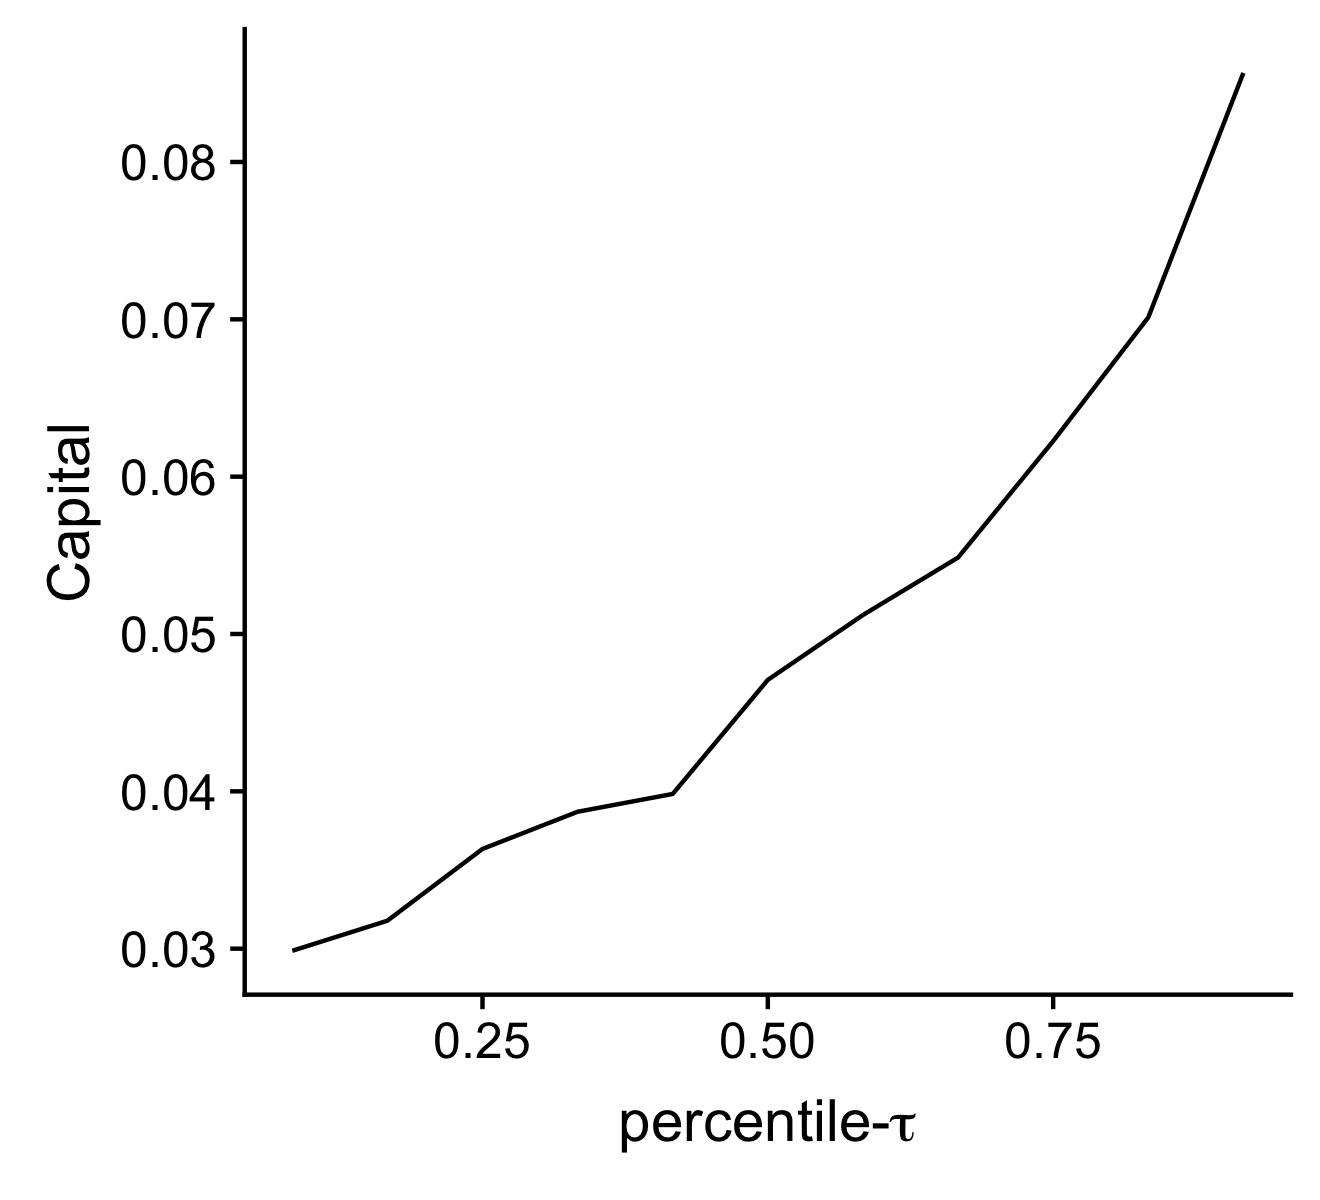
\includegraphics[width=9cm, height=9cm]{/Users/justindoty/Documents/Research/Dissertation/Nonlinear_Production_Function_QR/Code/Empirical/Results/Nonparametric/Translog/Plots/Elasticities/K_AQME.png}
\label{kaqme}
\end{figure} 

\begin{figure}[H]
\centering
\caption{Average Labor Elasticity}
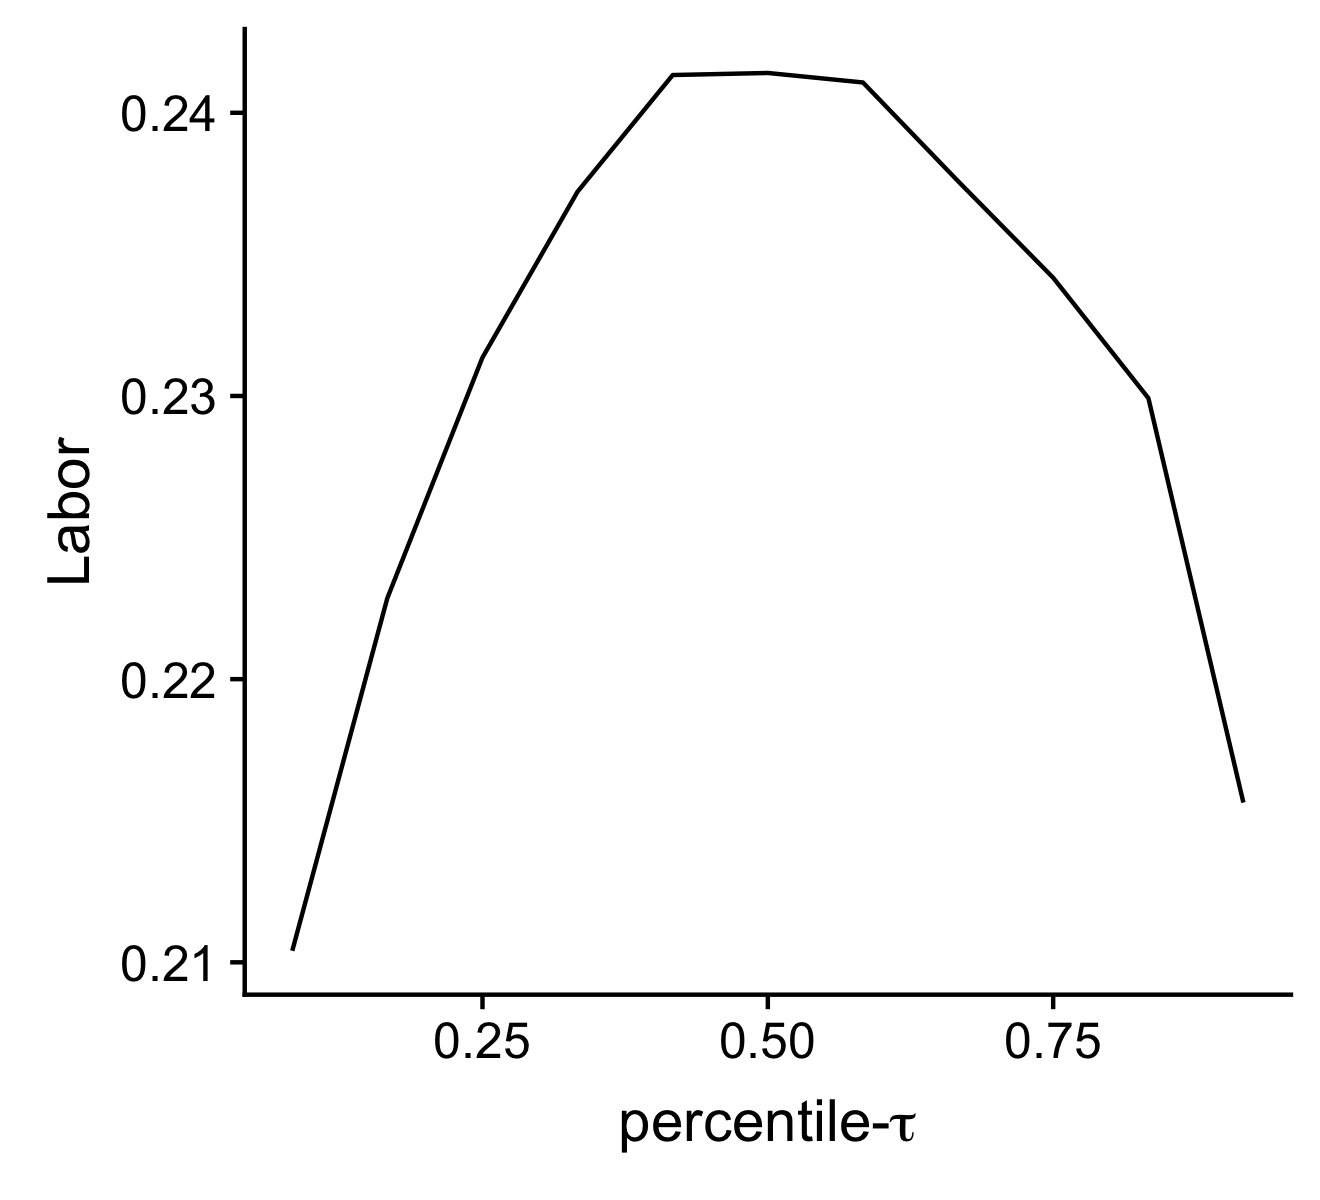
\includegraphics[width=9cm, height=9cm]{/Users/justindoty/Documents/Research/Dissertation/Nonlinear_Production_Function_QR/Code/Empirical/Results/Nonparametric/Translog/Plots/Elasticities/L_AQME.png}
\label{laqme}
\end{figure} 

\begin{figure}[H]
\centering
\caption{Average Materials Elasticity}
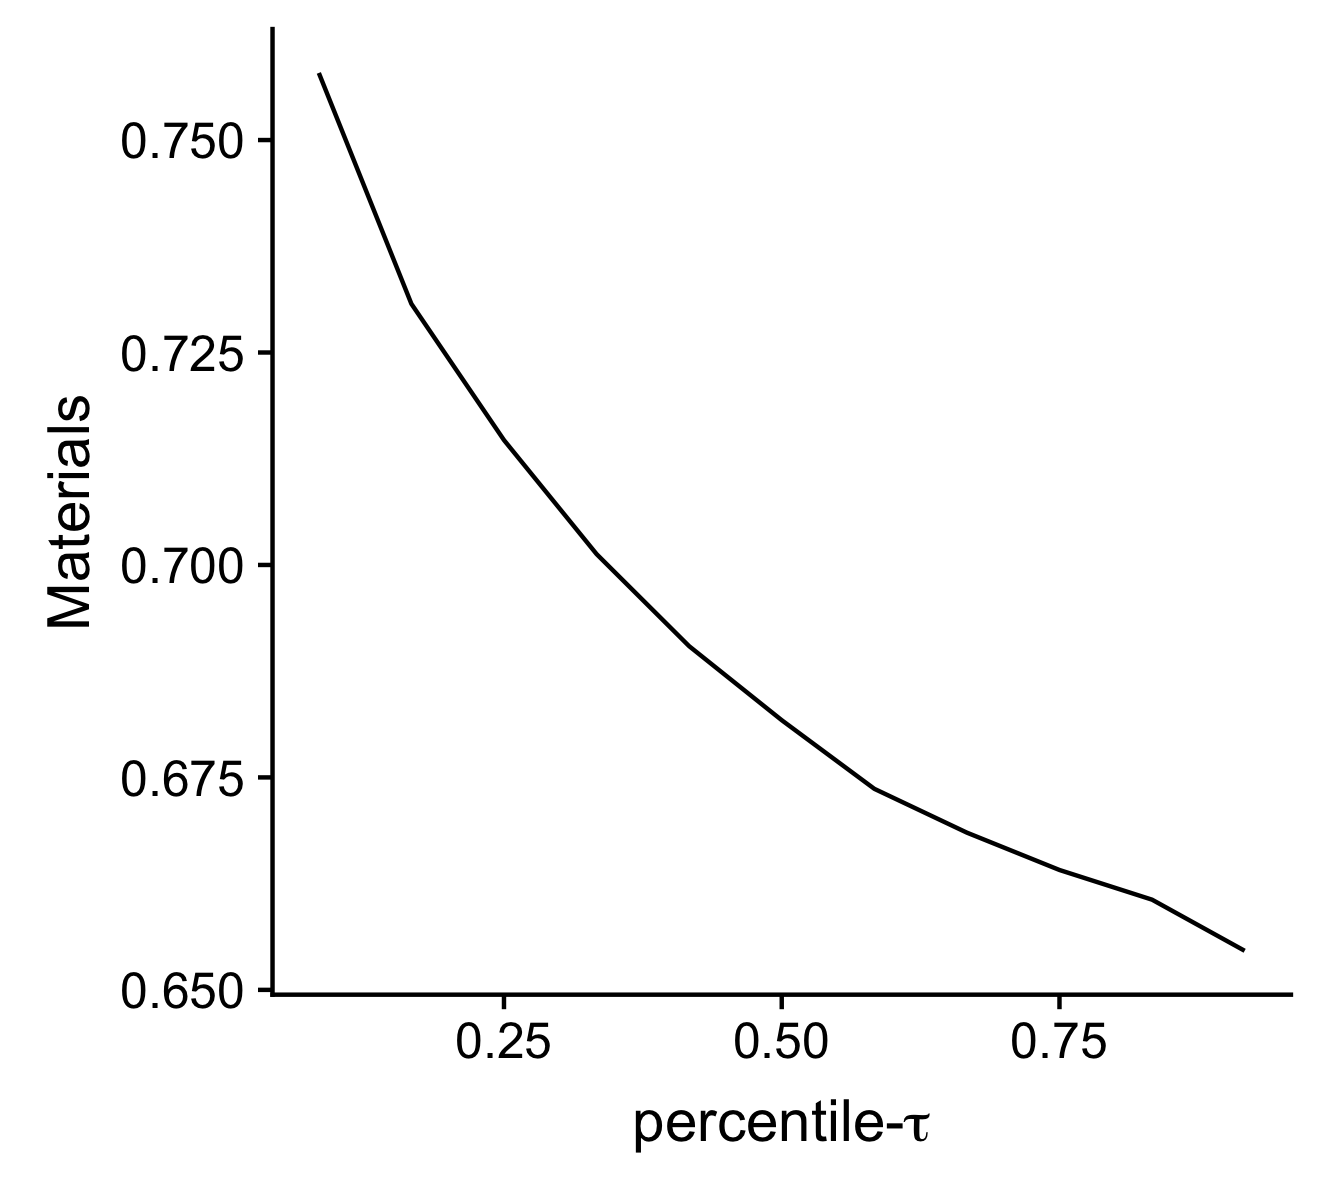
\includegraphics[width=9cm, height=9cm]{/Users/justindoty/Documents/Research/Dissertation/Nonlinear_Production_Function_QR/Code/Empirical/Results/Nonparametric/Translog/Plots/Elasticities/M_AQME.png}
\label{maqme}
\end{figure} 


\begin{figure}[H]
\centering
\caption{Average Capital-Productivity Effect}
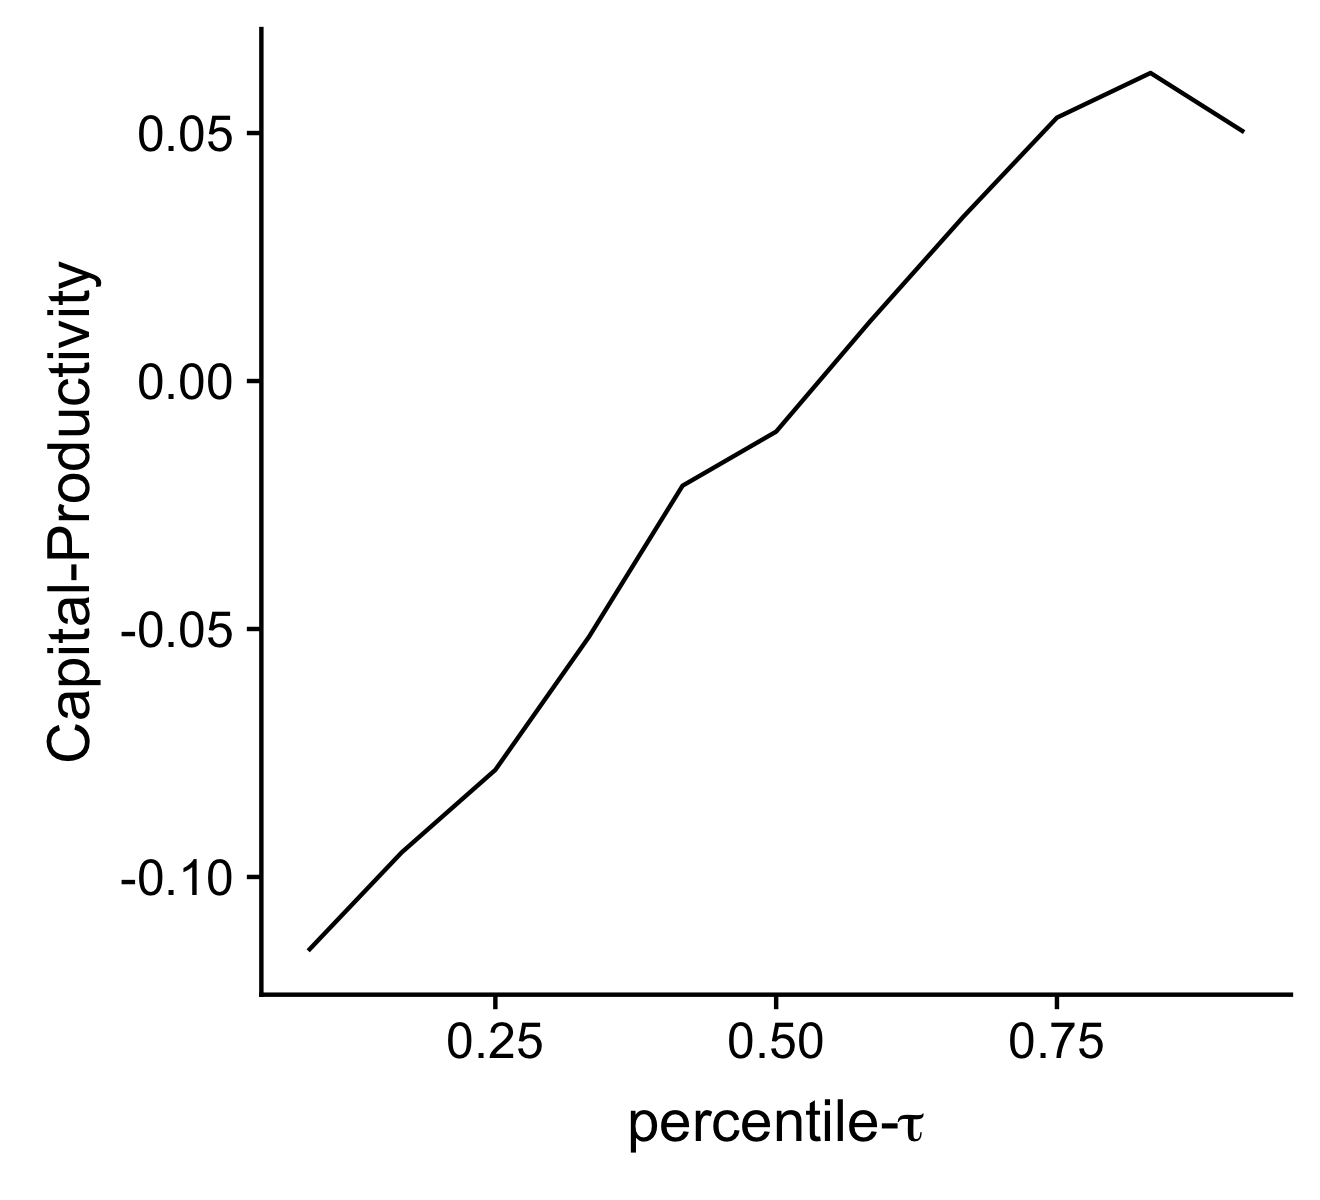
\includegraphics[width=9cm, height=9cm]{/Users/justindoty/Documents/Research/Dissertation/Nonlinear_Production_Function_QR/Code/Empirical/Results/Nonparametric/Translog/Plots/Hicks/HICKS_K_AQME.png}
\label{hkaqme}
\end{figure} 

\begin{figure}[H]
\centering
\caption{Average Labor-Productivity Effect}
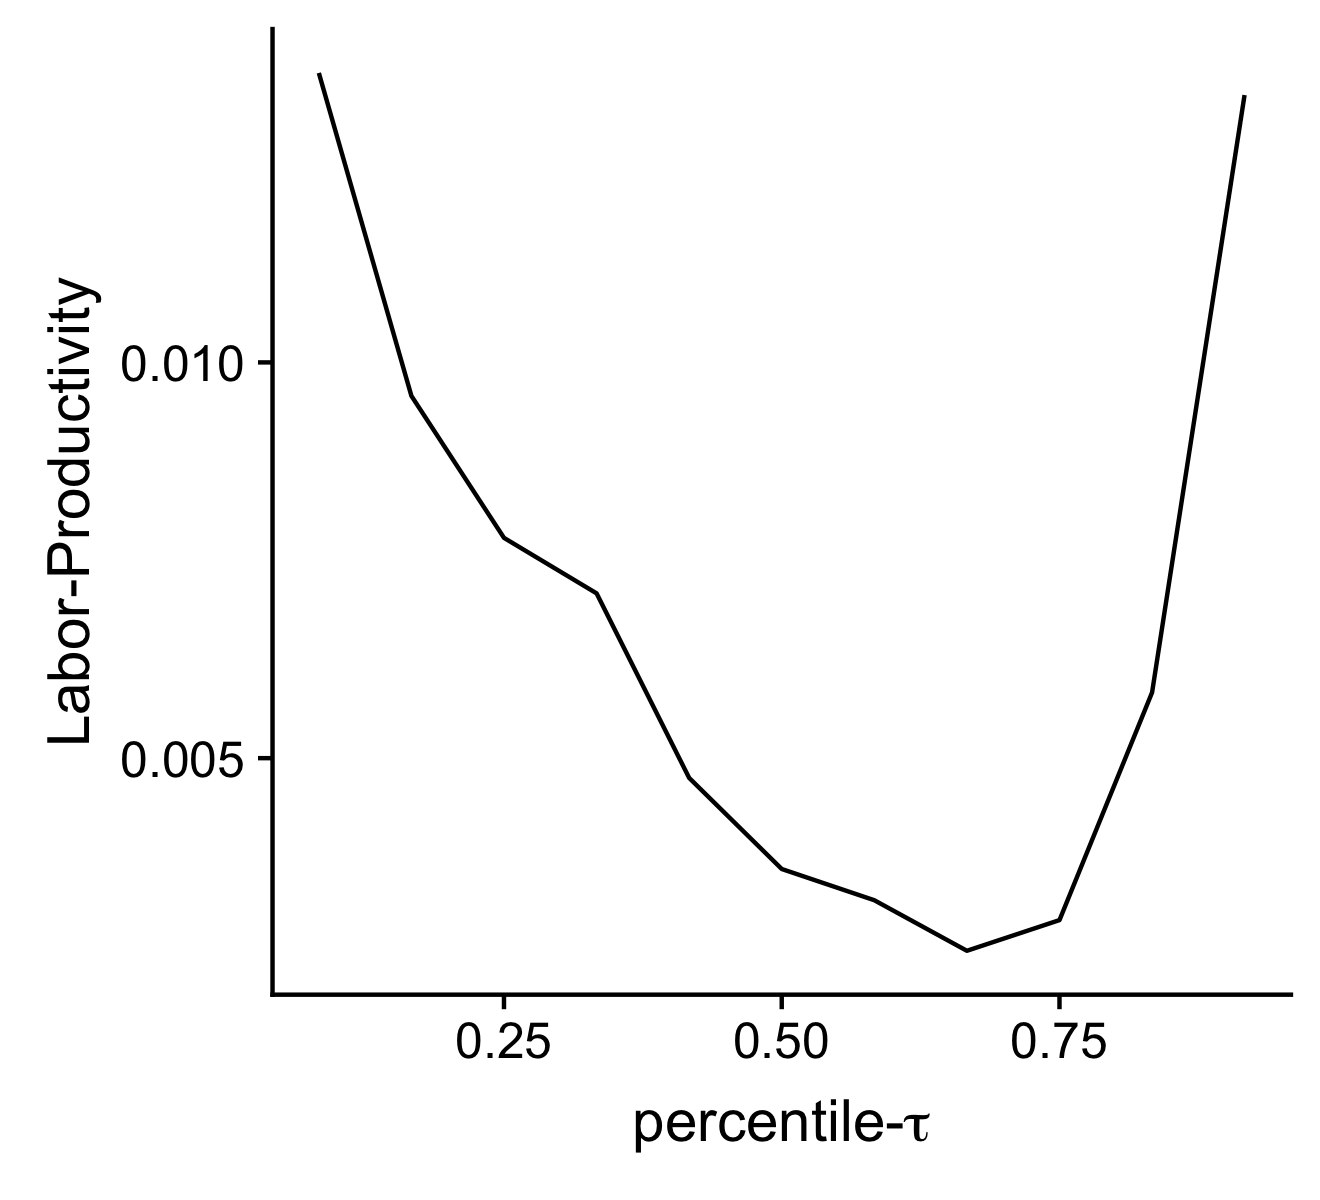
\includegraphics[width=9cm, height=9cm]{/Users/justindoty/Documents/Research/Dissertation/Nonlinear_Production_Function_QR/Code/Empirical/Results/Nonparametric/Translog/Plots/Hicks/HICKS_L_AQME.png}
\label{hlaqme}
\end{figure} 

\begin{figure}[H]
\centering
\caption{Average Materials-Productivity Effect}
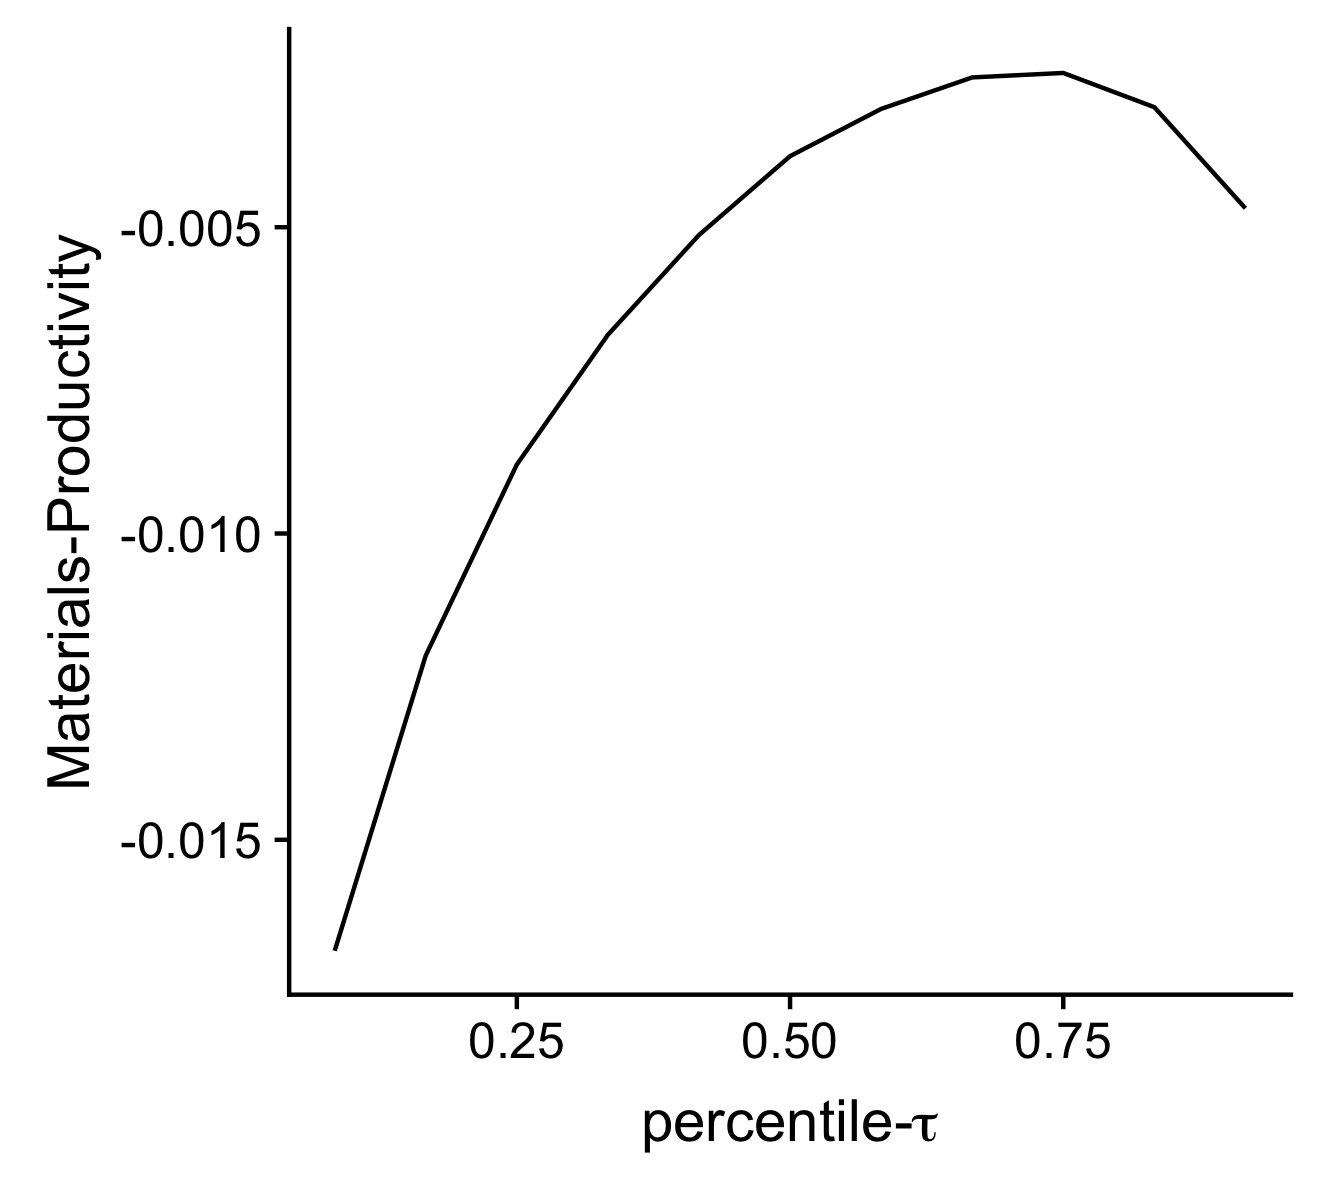
\includegraphics[width=9cm, height=9cm]{/Users/justindoty/Documents/Research/Dissertation/Nonlinear_Production_Function_QR/Code/Empirical/Results/Nonparametric/Translog/Plots/Hicks/HICKS_M_AQME.png}
\label{hmaqme}
\end{figure} 

\begin{figure}[H]
\centering
\caption{Average Persistence of Productivity}
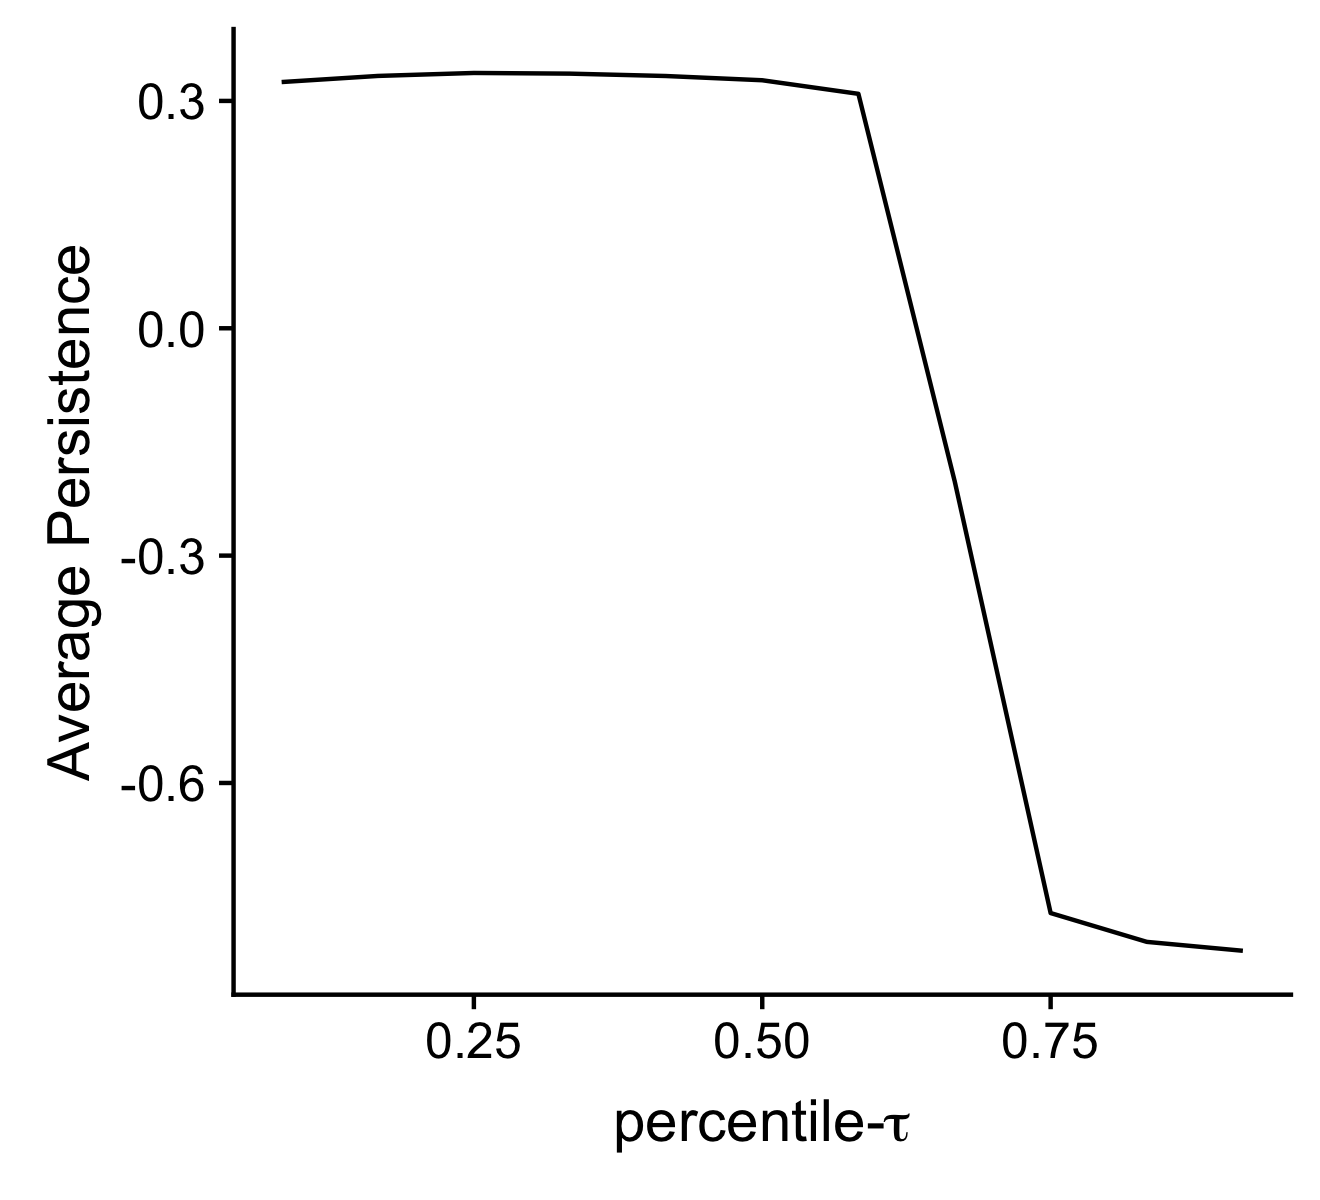
\includegraphics[width=9cm, height=9cm]{/Users/justindoty/Documents/Research/Dissertation/Nonlinear_Production_Function_QR/Code/Empirical/Results/Nonparametric/Translog/Plots/TFP/OMG_AQME.png}
\label{waqme}
\end{figure} 

\begin{figure}[H]
\centering
\caption{Distribution of Productivity}
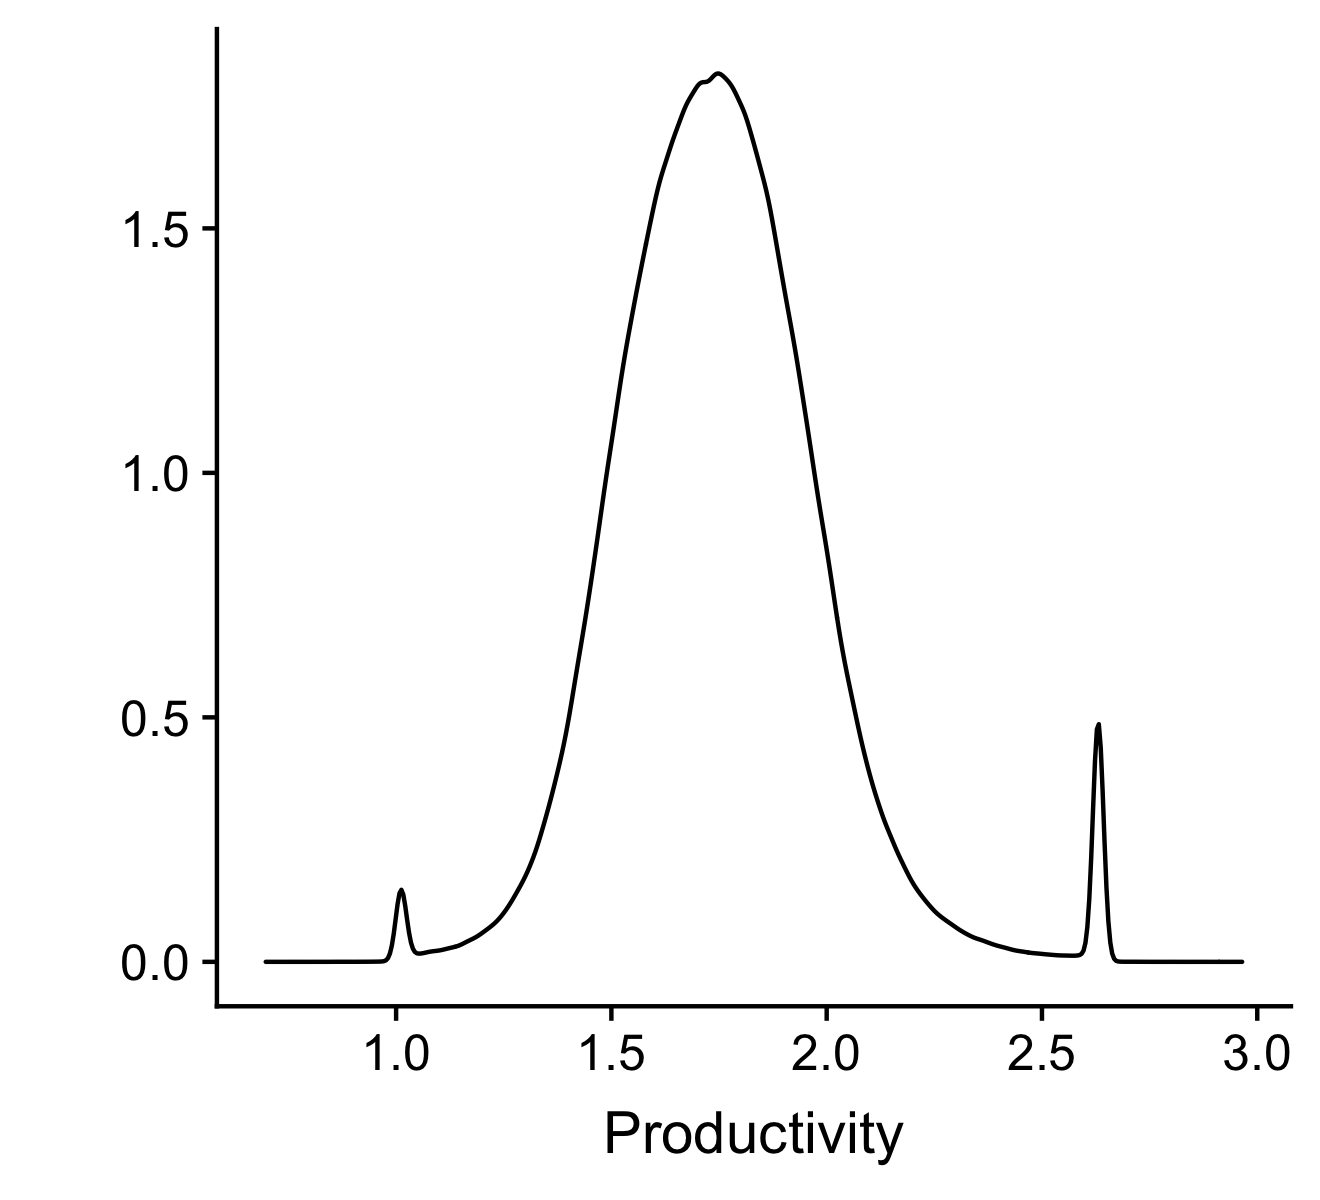
\includegraphics[width=9cm, height=9cm]{/Users/justindoty/Documents/Research/Dissertation/Nonlinear_Production_Function_QR/Code/Empirical/Results/Nonparametric/Translog/Plots/TFP/OMG_DENS.png}
\label{omgdens}
\end{figure} 





\pagebreak
\newpage
\bibliographystyle{ecca.bst}
\bibliography{NL_PF_QR}

\pagebreak
\newpage

\appendix

                                          







\end{document}